\section{Ziel}
In diesem Versuch soll die Lebensdauer kosmischer Myonen vermessen werden.
Mithilfe eines Szintillationsdetektors wird das Einfallen und der Zerfall der Myonen detektiert und die Zeitdifferenz vermessen.
Aus der gemessenen Zeitdifferenz lässt sich mithilfe von Regressionen die Lebensdauer der Myonen bestimmen.
\setcounter{page}{1}
\section{Theorie}
\label{sec:Theorie}
\subsection{Kosmische Myonen}
\label{sec:myonen}
Primäre Strahlung ist die Strahlung aus den astrophysikalischen Quellen, sie besteht hauptsächlich aus Protonen (ca \SI{85}{\percent}) und zu \SI{14}{\percent} aus Heliumkernen (S.\num{106} \cite{source1}).
In diesem Versuch werden die Myonen der sekundären kosmischen Strahlung untersucht.
Die Teilchen und die Strahlung, die bei der Wechselwirkung der primären kosmischen Strahlung mit der Atmosphäre entstehen, werden sekundäre kosmische Strahlung genannt.
Während bei den Zerfällen in der Atmosphäre viele verschiedene Teilchen erzeugt werden, sollen hier kosmische Myonen untersucht werden.
Etwa \SI{80}{\percent} der hier untersuchten Strahlung auf Meereshöhe besteht aus Myonen (S. \num{208} \cite{source1}), der Fluss der Elementarteilchen an der Erdoberfläche beträgt dabei ein Teilchen pro \si{\square \centi \metre} .
Myonen bilden zusammen mit den Myon-Neutrinos die 2. Lepton-Generation.
Die Elementarteilchen haben eine Ladung von \SI{-1}{\elementarycharge} und eine Masse von \SI[per-mode=symbol]{0.106}{\giga \eV \per \clight \squared} (S. \num{30} \cite{source1}).

In einer Höhe von \num{15} bis \SI{20}{\kilo\metre} entstehen durch das einfallen hochenergetischer Protonen die hadronischen und elektromagnetischen Schauer der primären kosmischen Strahlung.
In diesen Schauern werden neben vielen anderen Teilchen auch Pionen erzeugt die gemäß Abbildung \ref{fig:entstehung} Myonen erzeugen.

\begin{figure}
    \begin{subfigure}{0.5\textwidth}
        \centering
        \feynmandiagram [horizontal=a to b] {
        i1 [particle=\(u\)] -- [fermion] a -- [fermion] i2 [particle=\(\overline d\)],  
        a -- [boson, edge label'=\(W^{+}\)] b,
        f1 [particle=\(\mu^{+}\)] -- [fermion] b -- [fermion] f2 [particle=\(\nu_{\mu}\)], 
        };
    \end{subfigure}
    \begin{subfigure}{0.5\textwidth}
        \centering
        \feynmandiagram [horizontal=a to b] {
        i1 [particle=\(d\)] -- [fermion] a -- [fermion] i2 [particle=\(\overline u\)],  
        a -- [boson, edge label'=\(W^{-}\)] b,
        f1 [particle=\(\overline \nu_{\mu}\)] -- [fermion] b -- [fermion] f2 [particle=\(\mu^{-}\)], 
        };
    \end{subfigure}
    \caption{Die beiden Hauptkanäle für die Entstehung der Myonen. Die Zerfälle sind sowohl mit Pionen als auch Kaonen in ähnlicher Form möglich, allerdings mit Kaonen deutlich seltener.}
    \label{fig:entstehung}
\end{figure}

Die erzeugten Myonen bewegen sich mit hohen Geschwindigkeiten zur Erdoberfläche und können dort Nachgewiesen werden.
Während ihrer propagation können die Myonen jeden Moment gemäß der Prozesse Abbildung \ref{fig:zerfall} zerfallen.
\begin{figure}
    \begin{subfigure}{0.5\textwidth}
        \centering
        \feynmandiagram [layered layout, horizontal=a to b] {
        a [particle=\(\mu^{-}\)] -- [fermion] b -- [fermion] f1 [particle=\(\nu_{\mu}\)],
        b -- [boson, edge label'=\(W^{-}\)]c,
        c -- [anti fermion] f2 [particle=\(\overline \nu_{e}\)],
        c -- [fermion] f3 [particle=\(e^{-}\)],
        };
    \end{subfigure}
    \begin{subfigure}{0.5\textwidth}
        \centering
        \feynmandiagram [layered layout, horizontal=a to b] {
        a [particle=\(\mu^{+}\)] -- [anti fermion] b -- [anti fermion] f1 [particle=\(\overline \nu_{\mu}\)],
        b -- [boson, edge label'=\(W^{+}\)] c,
        c -- [anti fermion] f2 [particle=\(e^{+}\)],
        c -- [fermion] f3 [particle=\(\nu_{e}\)],
        };
    \end{subfigure}
    \caption{Die Hauptkanäle des Myon-Zerfalls.}
    \label{fig:zerfall}
\end{figure}

\subsection{Detektion}
\label{sec:szintillator}
Die kosmischen Myonen werden mithilfe eines Szintillators auf der Erdoberfläche detektiert.
Der Prozess der Szintillation beschreibt die erzeugung von Licht mit einem charakteristischen Spektrum durch die Absorption von ionisierender Strahlung (S.\num{495} \cite{source2}).
Szintillation kann durch zwei verschiedene Mechanismen entstehen. 
Zum einen kann ein Atom durch die Strahlung ionisiert werden und bei der anschließenden Rekombination Licht aussenden.
Zum anderen kann ein Atom angeregt werden und beim Wechsel zurück in einen niedrigeren Energiezustand ein Photon aussenden.
In beiden Fällen wird das erzeugte Licht mit Photovervielfachern (Photomultiplier Tube, PMT \ref{sec:pmt}) gemessen und der Spannungsimpuls ausgelesen.

Szintillatoren werden in zwei Gruppen gemäß ihrer Funktionsweise aufgeteilt, organische und anorganische Szintillatoren.

\begin{description}
    \item[Organische Szintillatoren] arbeiten mithilfe der Energieniveaus der Kohlenstoffatome. Bei Anregung des Atoms wird dieses vom Grundzustand $\text{S}_{00}$ auf höhere Niveaus gebracht. Beim direkten zurückfallen auf den Grundzustand entsteht prompte Fluoreszenz.
    \item[Anorganische Szintillatoren] funktionieren mithilfe der Gitterstruktur von Kristallen. Durch einfallende Strahlung werden Elektronen vom Valenzband in das Leitungsband angehoben. Mit der erhöhten Energie fällt das Elektron anschließend in ein Potentialminimum ad und gibt beim Übergang vom Potentialminimum auf das Valenzband ein Photon ab. 
\end{description}

Die beiden Arten von Szintillatoren haben verschiedene Vorteile und daher verschiedene Einsatzbereiche.
Da in diesem Versuch eine messung der Lebensdauer der Myonen und somit eine zeitkritische Messung durchgeführt erden soll eignet sich ein Organischer Szintillator besser.

Der Szintillator in diesem Aufbau besteht aus einem liegenden, zylinderförmigen Tank der lichtundurchlässig verschlossen ist.
Der Tank ist mit \SI{50}{\litre} organischen, gelösten Szintillat gefüllt zur Detektion der Myonen.
An beiden Seiten des Zylinders befindet sich jeweils ein PMT zur Messung der Photonenimpulse.
Die beiden PMTs sind mit der in Kapitel \ref{sec:Durchfuehrung} beschriebenen Schaltung verbunden.

\subsubsection{Photovervielfacher}
\label{sec:pmt}
Photovervielfacher sind eine weit verbreitete Methode Photonen zu messen.
Ein PMT besteht im Grundsatz aus drei Teilen, der Photokathode, einem Verstärker und der Anode wie in Abbildung \ref{fig:pmt} dargestellt.
Ein Photon fällt durch die Glasabdeckung des PMT ein und löst durch den Photoeffekt (Kap.3.5.2 \cite{source2}) Elektronen aus der aufgedampften Photokathode aus.
Die ausgelösten Photonen werden durch eine Blende auf die Dynoden des Verstärkersystems gelenkt.
Mit den Dynoden werden die Photonen durch ausgelöste Sekundärelektronen bis zu \num{1e5} bis \num{1e9} fach verstärkt (S. \num{414} \cite{source2}).
Das verstärkte Signal kann beim eintreffen an der Anode als elektrischer Puls ausgelesen werden (\cite{source2}).
\begin{figure}[ht]
    \centering
    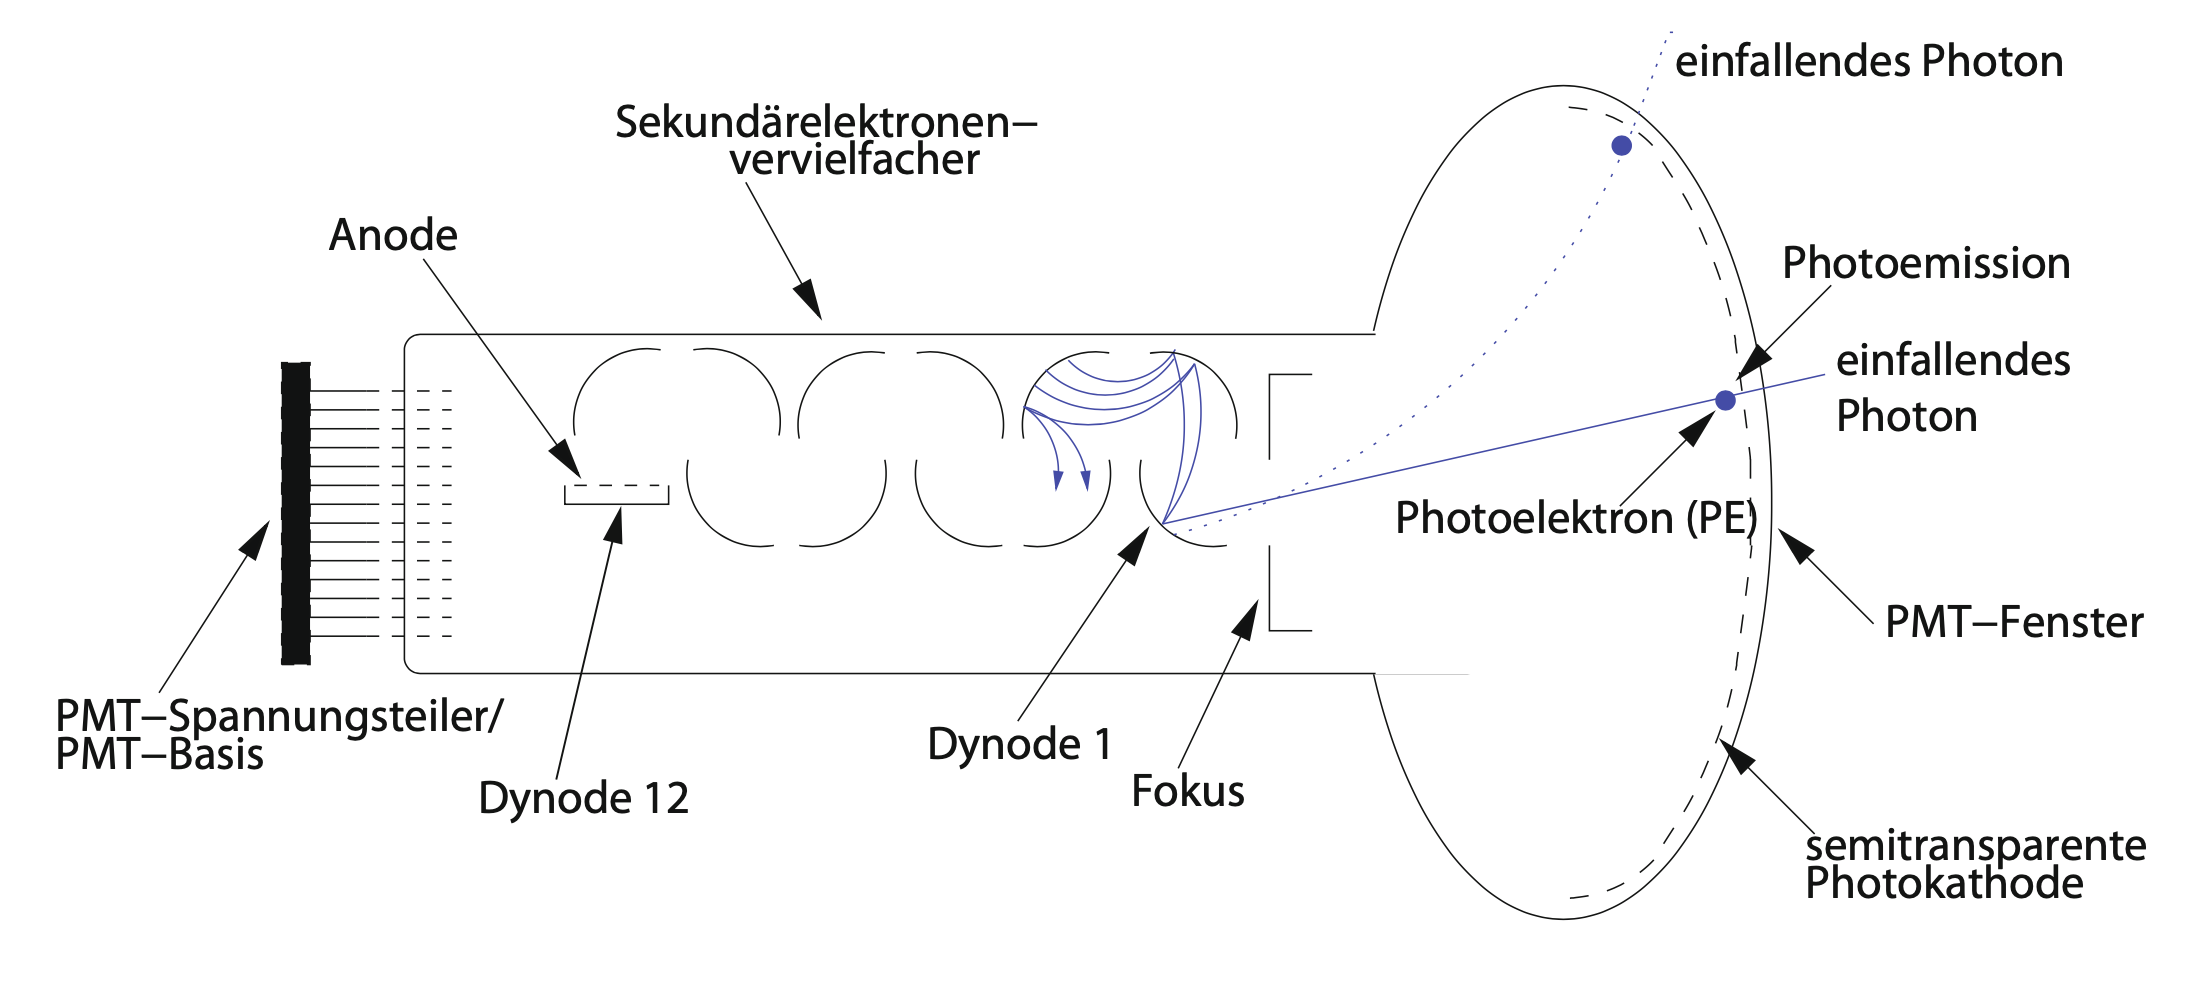
\includegraphics[width = \textwidth]{./bilder/PMT.png}
    \caption{Funktionszeichnung eines PMT. Über die Kathode fällt licht ein und löst Elektron aus. Durch den Fokus fallen die Elektronen auf die Dynoden und nach der Verstärkung auf die Anode. Die Spannung für die verschiedenen Bauteile wir über eine Basisplatte am ende des PMT bereitgestellt \cite{Schmidt2002Aufbau}.}
    \label{fig:pmt}
\end{figure}

\subsection{Vorbereitung}
\subsubsection{Was definiert die Lebensdauer und aus welchem Zusammenhang lässt sie sich herleiten?}
Die Lebensdauer kosmischer Myonen wird durch ihren Zerfall und daher durch das exponentielle Zerfallsgesetz definiert.
\begin{align*}
    \frac{1}{e} N_0 &= N_0 e^{-\frac{\Gamma}{\hbar} t}\\
    e^{-1} &= e^{-\frac{\Gamma}{\hbar} t}\\
    1 &= \frac{\Gamma}{\hbar} t \\
    t &= \frac{\hbar}{\Gamma}
\end{align*}
\subsubsection{Berechnen sie klassich und relativistisch aus der Sicht eines auf der Erde ruhenden Beobachters die Reichweite eines kosmischen Myons.}
\begin{align*}
    E_{\mu} &= \SI{10}{\giga \electronvolt}\\
    E^2 &= m^2c^2 + p^2c^2 \\
    v &= c\sqrt{1-\frac{m^2 c^4}{E^2}}\\
    s &= v\tau = \tau c \sqrt{1-\frac{m^2 c^4}{E^2}} = \SI{659.5}{\metre}\\
    s\prime &= \frac{s}{\gamma} = \SI{659.5}{\metre} \sqrt{1-\frac{v^2}{c^2}} = \SI{62418}{\metre}
\end{align*}
\subsubsection{Welche Ereignisrate erwarten Sie auf der Erdoberfläche? Den Szintillatortank können Sie als liegenden Zylinder nähern.}
Die Myonen werden als senkrecht auf den Szintillator treffend angenommen und die Fläche des Tanks ergibt sich damit zu $A = 2hr$.
Auf der Erdoberfläche beträgt der Myonenfluss circa \SI{1}{\per \square \centi \metre \per \minute}.
\begin{align*}
    \SI{1}{\per \square \centi \metre \per \minute} &= \SI{166.7}{\per \square \metre \per \second} \\
    \pi h r^2 &= 2\pi r^3 = \SI{0.05}{\cubic \metre} \\
    r &≈ \SI{0.1996}{\meter} \\
    h &= 2r \\
    \text{Ereignisrate} &= \SI{166.7}{\per \square \metre \per \second} \cdot 4r^2 \\
    &= \SI{1595}{\per \minute} \\
    &= \SI{26.58}{\hertz}
\end{align*}